\documentclass[nobib]{tufte-handout}

\title{Lecture 2: Eulerianity, simple graphs, and subgraphs $\cdot$ 1MA020}

\author[Vilhelm Agdur]{Vilhelm Agdur\thanks{\href{mailto:vilhelm.agdur@math.uu.se}{\nolinkurl{vilhelm.agdur@math.uu.se}}}}

\date{24 October 2023}


%\geometry{showframe} % display margins for debugging page layout

\usepackage{graphicx} % allow embedded images
  \setkeys{Gin}{width=\linewidth,totalheight=\textheight,keepaspectratio}
  \graphicspath{{graphics/}} % set of paths to search for images
\usepackage{amsmath}  % extended mathematics
\usepackage{booktabs} % book-quality tables
\usepackage{units}    % non-stacked fractions and better unit spacing
\usepackage{multicol} % multiple column layout facilities
\usepackage{lipsum}   % filler text
\usepackage{fancyvrb} % extended verbatim environments
  \fvset{fontsize=\normalsize}% default font size for fancy-verbatim environments

\usepackage{color,soul} % Highlights for text

% Standardize command font styles and environments
\newcommand{\doccmd}[1]{\texttt{\textbackslash#1}}% command name -- adds backslash automatically
\newcommand{\docopt}[1]{\ensuremath{\langle}\textrm{\textit{#1}}\ensuremath{\rangle}}% optional command argument
\newcommand{\docarg}[1]{\textrm{\textit{#1}}}% (required) command argument
\newcommand{\docenv}[1]{\textsf{#1}}% environment name
\newcommand{\docpkg}[1]{\texttt{#1}}% package name
\newcommand{\doccls}[1]{\texttt{#1}}% document class name
\newcommand{\docclsopt}[1]{\texttt{#1}}% document class option name
\newenvironment{docspec}{\begin{quote}\noindent}{\end{quote}}% command specification environment

\include{mathcommands.extratex}

\begin{document}

\maketitle% this prints the handout title, author, and date

\begin{abstract}
\noindent
We formalize the ideas we started with in the first exercise session, giving a proof of Euler's result on Eulerian circuits. We then make some more definitions about simple graphs and subgraphs, and we state some elementary results about these notions.
\end{abstract}

The very first definition we give in this course will actually be of a \emph{multigraph}, not the simple graphs that were our first example.\sidenote[][-0.7cm]{These are of course a type of graph, so we will often just write or say ``graph'' when it is clear from context what type of graph we are referring to, or what we are saying applies to any type of graph.}

\begin{definition}
    A \emph{multigraph} $G$ is a tuple $(V, E)$, consisting of a set $V$ of \emph{vertices}, and a multiset\sidenote[][]{A multiset is just like a set, except an element may occur more than once.} $E$ of \emph{edges}. Each edge is a multiset containing two vertices from $V$, called its \emph{endpoints}. We say two vertices are \emph{adjacent} if there is an edge between them, and a vertex $v$ is \emph{incident} to an edge $e$ if $v \in e$.

    If the same edge occurs more than once in $E$, we say that these edges are \emph{parallel}. If the two endpoints of an edge are equal, we call it a \emph{loop}.

    Unless explicitly stated, we always assume that both $V$ and $E$ are finite sets. Otherwise, we say the graph is \emph{infinite}.\sidenote[][]{It may sometimes be the case that our proofs work without modification also for infinite graphs -- thinking about whether they do may be a useful thing to do when reading the proofs, to understand them better.}
\end{definition}

Next, continuing to formalize the things we learned thinking about the bridges of Königsberg, let us define what a walk is.

\begin{definition}
    Let $G = (V, E)$ be a multigraph. A \emph{walk} of length $k$ is a sequence of $k+1$ vertices $v_0 v_1 v_2\ldots v_k$ and a sequence of $k$ edges\sidenote[][]{So the length of a walk is the number of edges, not the number of vertices.} $e_1e_2\ldots e_k$ such that $e_i = \{v_{i-1}, v_i\}$ for all $i$. A \emph{trail} is a walk that uses no edge twice, and a \emph{path} is a walk that uses no vertex twice. A \emph{circuit} is a trail where the first and last vertices coincide, and a \emph{cycle} is a circuit where these are the only vertices that coincide.
\end{definition}

\begin{figure}
    \centering
    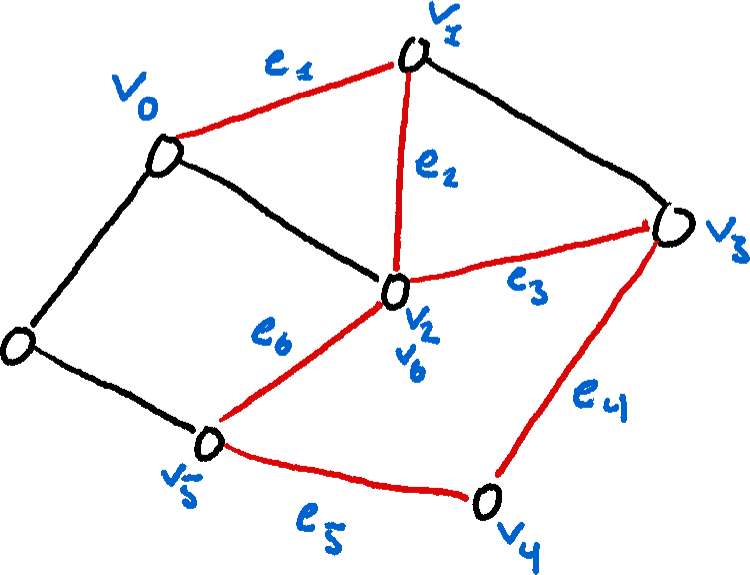
\includegraphics[width=0.7\textwidth]{graphics/L2_eulerianity_subgraphs/walk_in_graph.png}
    \caption[][0cm]{A walk in a graph, which is a trail but not a path.}
    \label{fig:walk_in_graph}
\end{figure}

We have one example of a walk in Figure \ref{fig:walk_in_graph} -- it does not repeat any of the edges, so it is a trail, but it repeats the central vertex we have labelled with both $v_2$ and $v_6$, so it is not a path.

Having introduced walks, we can give a definition of another very natural property, namely connectedness.\sidenote[][]{You've probably already seen the notion of connectedness of a subset of $\R^2$ in a calculus course, and if you've looked at other geometry it appears there as well. This is the same notion, just discretized.}

\begin{definition}
  We say that a graph $G$ is \emph{connected} if there is, for any two vertices $u, v \in G$, a walk from $u$ to $v$. We say that two vertices in a graph are connected to each other if there is a walk between them.

  Notice that there is a trivial ``lazy'' walk connecting every vertex to itself, so the relation of connectedness is an equivalence relation. The equivalence classes of this equivalence relation are called the \emph{connected components} of the graph.\sidenote[][]{We could equivalently have defined the connected components as the maximal connected subgraphs of the graph -- when we get to a formal definition of subgraph, think about why this is true.}
\end{definition}

Let us now define the thing we were studying when we thought about the bridges of Königsberg.

\begin{definition}
  An \emph{Eulerian trail} is a trail that uses every edge in the graph exactly once -- if additionally it has the same starting and ending vertex, we call it an \emph{Eulerian circuit}. If there is an Eulerian circuit in a graph, we call the graph \emph{Eulerian}.
\end{definition}

The problem we were studying was thus to find a simple condition for when a multigraph is Eulerian. The condition we found\sidenote[][]{Hopefully.} involved the number of edges incident to a vertex, so let us also give this notion a name.

\begin{definition}
  The \emph{degree} of a vertex $v$, denoted $d_v$, is the number of edges a vertex is incident to, with loops counted twice.
\end{definition}

We now have all the language we need to formally state and prove the theorem that started graph theory all those nearly three hundred years ago.

\begin{theorem}[Euler (1736)]
  A finite connected multigraph is Eulerian if and only if all its vertices have even degree.

  \begin{proof}
    Let us begin with the easy direction of this statement: That a graph which is Eulerian will have only even-degree vertices. To see this, note that the Eulerian circuit gives us a way to pair up the edges incident to any vertex -- the path enters through one edge and leaves through another, so we pair those up. Since the circuit uses every edge, there can't be any odd edge left over in this pairing, and so the degree of the vertex can't be odd.

    So, for the harder direction, we will prove the result by induction on the number of edges.\sidenote[][]{This is a different proof than the one given in the lecture notes from last year. The reason for changing the proof is that I couldn't understand what was going on in the previous proof. Feel free to look at the other proof if this one doesn't make sense to you -- maybe it will.} The base case is $n=0$, where the graph must just be a single vertex. That this is Eulerian is trivial -- the lazy path that does nothing uses every edge in the graph, since the graph has no edges.

    Now, let $G = (V,E)$ be a finite connected multigraph with only even vertex degrees, with $n \geq 1$ edges. Pick an arbitrary vertex $v$, then pick an arbitrary edge $e = \{v, w\}$ going out from $v$.\sidenote[][]{This edge is allowed to be a loop -- think about what happens in that case.} Then pick another edge going out from $w$, making sure it hasn't already been used in our path, and so on, until you have returned to $v$. Let $W$ be the set of edges we used in this walk.

    That we will always be able to pick an unused edge to continue walking along follows from our assumption that the degrees of vertices are even -- if we were able to use an edge to get to a vertex we must also be able to pick one to leave it, since we always use up edges in pairs.
    
    \begin{figure}
      \centering
      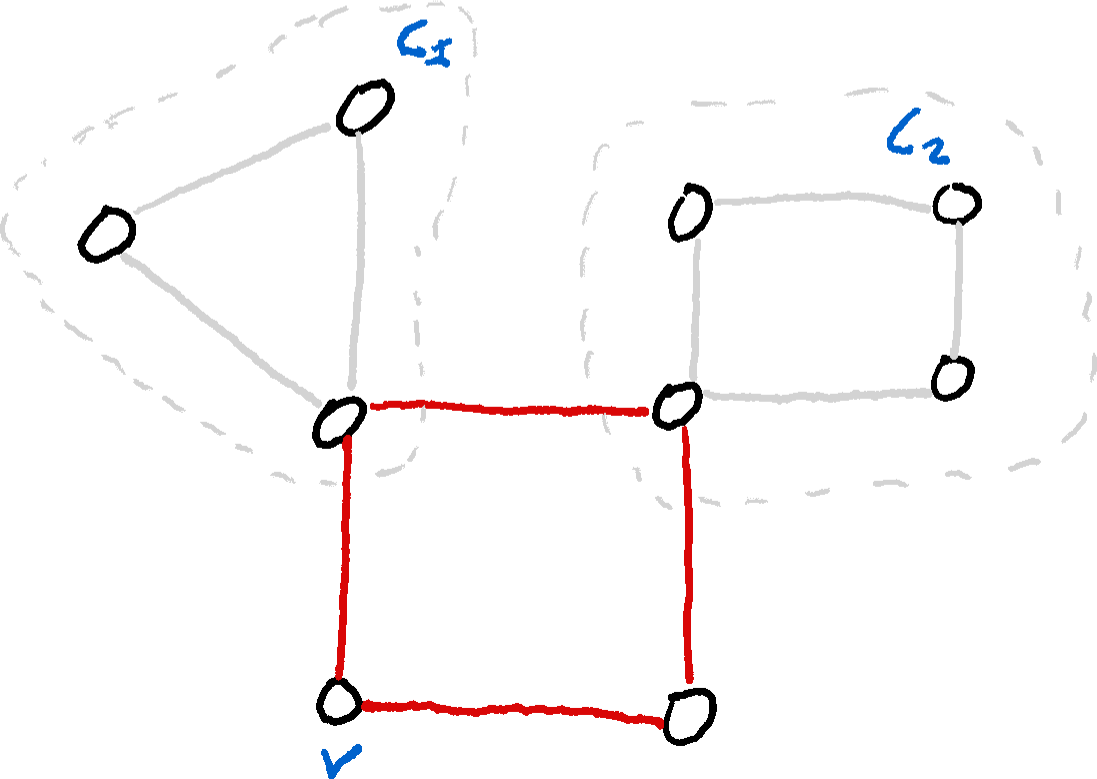
\includegraphics[width=0.7\textwidth]{graphics/L2_eulerianity_subgraphs/eulerianity_connected_components.png}
      \caption[][0cm]{A graph $G = (V,E)$ with the path $W$ highlighted in red, and the two connected components $C_1$ and $C_2$ of $H = (V, E \setminus W)$ indicated.}
      \label{fig:euler_proof_connected_components}
    \end{figure}

    Now consider the graph $H = (V, E \setminus W)$, that is, $G$ with all the edges we used in our walk removed. Let $C_1, C_2, \ldots, C_k$ be its connected components, as is illustrated in Figure \ref{fig:euler_proof_connected_components}. Now, each of these components necessarily has fewer than $n$ edges, and is of course trivially connected, so by our induction hypothesis each contains an Eulerian circuit.

    The idea now is to glue together our circuit $W$ with the circuits on the $C_i$ to get an Eulerian circuit on the entire graph. To do this, what we need is that each $C_i$ contains at least one vertex that is incident to an edge in $W$.

    To see this,\sidenote[][]{This is the hardest piece of the proof -- at least in the sense that it is hard to write in a way that is both rigorous and understandable. Once it ``clicks'' why this should be true, it is hopefully less hard. The figure, and the lecture, might help.} pick a connected component $C_i$. If $v \in C_i$, we are done, so assume it is not. We now pick some arbitrary vertex $w$ in $C_i$ -- since $G$ is by assumption connected, there exists a walk connecting $w$ to $v$. Since $v$ is not in $C_i$, this walk must at some point leave $C_i$ -- so consider the edge it leaves $C_i$ by, say, $e = \{a,b\}$, walking from $a \in C_i$ to $b \not\in C_i$. This edge must in fact be in $W$, because if it weren't, it'd be an edge of $H$, and $a$ is in $C_i$ -- and thus $b$ would also be in $C_i$, by definition of connected component, and this edge wouldn't be leaving $C_i$ at all. So the vertex $a$ must both be in $C_i$ and be incident to an edge of $W$.

    \begin{figure}
      \centering
      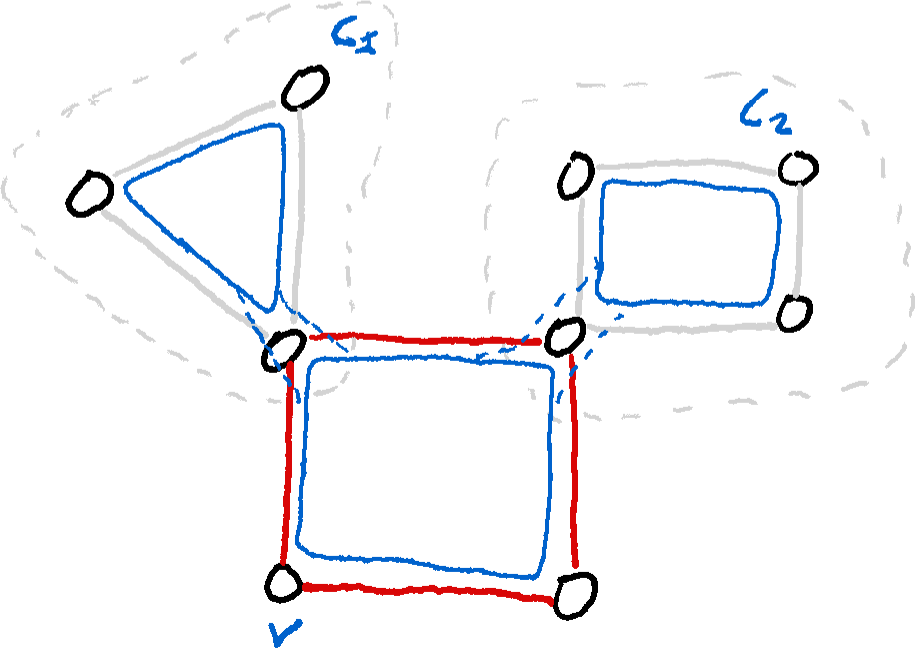
\includegraphics[width=0.7\textwidth]{graphics/L2_eulerianity_subgraphs/eulerianity_gluing_circuits.png}
      \caption[][0cm]{A graph $G = (V,E)$ with the path $W$ highlighted in red, and the two connected components $C_1$ and $C_2$ of $H = (V, E \setminus W)$ indicated. Additionally, the Eulerian circuits on the connected components and $W$ are drawn in blue, and their gluing together in dashed blue lines.}
      \label{fig:gluing_eulerian_circuits}
    \end{figure}

    So, for each $C_i$, let $a_i$ be a vertex in $C_i$ incident to an edge in $W$. We construct our Eulerian circuit on $G$ as follows: Start at $v$ and walk along $W$. Whenever you encounter an $a_i$, instead follow the Eulerian circuit in $C_i$ all the way around until you return to this $a_i$, and then proceed along $W$. That this will produce an Eulerian circuit on the entire graph should be clear, as is illustrated in Figure \ref{fig:gluing_eulerian_circuits}.
  \end{proof}
\end{theorem}

If we didn't require the trail to start and end at the same vertex, we could get away with having the start- and endpoint have odd degree. Let us state this as a corollary:

\begin{corollary}
  A finite connected graph admits an Eulerian trail if and only if either $0$ or $2$ of its vertices have odd degree.

  \begin{proof}
    If all vertices have even degree, this is just the theorem we just proved. If there are two vertices of odd degree, connect them with a new edge, so they both have even degree, and apply the theorem.
  \end{proof}
\end{corollary}

It is perhaps a bit misleading to attribute the entire theorem to Euler -- he stated it, but he only proved the easy direction. One thing he reportedly \emph{did} write a proof of is the so-called ``handshake lemma'', which also lets us settle the question of what happens if there is exactly one vertex of odd degree.

\begin{lemma}[Handshake lemma]
  Let $G = (V,E)$ be a finite graph. Then
    $$2\abs{E} = \sum_{v \in V} d_v.$$

  \begin{proof}
    To see this, we use the method of \emph{double counting} -- that is, we count one thing in two different ways. The thing we are going to count is \emph{half-edges}, that is, edges going out of vertices.\sidenote[][]{Imagine taking a pair of scissors to each edge, cutting them in half, to motivate the term. You can then recover a graph by pairing up half-edges into edges.}

    On the one hand, each edge obviously contributes two half-edges, so there are $2\abs{E}$ in the entire graph. On the other hand, each vertex contributes precisely its degree to the count of half-edges, so there are $\sum_{v\in V} d_v$ of them, proving the lemma.
  \end{proof}
\end{lemma}

\begin{corollary}
  Any graph must have an even number of odd-degree vertices.
  \begin{proof}
    The sum of the degrees must, by the handshake lemma, be even, and the sum of an odd number of odd numbers is odd.
  \end{proof}
\end{corollary}

%\bibliography{references}
%\bibliographystyle{plainnat}

\end{document}
